%%%%%%%%%%%%%%%%%%%%%%%%%%%%%%%%%%%%%%%%%%%%%%%%%%%%%%%%%%%%%%%%%%%%%%%%%%%%%%%%%
%%%%%                                RESULTS                                 %%%%
%%%%%%%%%%%%%%%%%%%%%%%%%%%%%%%%%%%%%%%%%%%%%%%%%%%%%%%%%%%%%%%%%%%%%%%%%%%%%%%%%

In this section we present our main results. In all cases standard errors are clustered at the 
state level so to match the main source of variation of the MW changes. We initially show how the 
estimated elasticity of rents to MW is approximately 0.026 when adopting the \textit{static DiD} 
model. We  check for the presence of unobserved time-varying factors systematically affecting changes 
in MW and rents that may confound our estimates. We progressively 
include controls for the local economy and the labor market, and we show how results 
do not change. We further show how the introduction of zipcode-level linear and quadratic 
trend leaves our results unchanged.  We then present estimates for the \textit{dynamic} models 
(\autoref{eq:leads_lags}) that highlight both the absence 
of pre-trends, and the presence of a 2-months dynamic effect: we estimate the cumulative impact of a 10 percent MW 
change to be between 0.5 and 0.6 percent over the course of the 5 months after the policy 
change. Since we don't observe changes in the underlying composition of rental listings on Zillow, 
identification may be threatened by a systematically different impact of MW on the number of listings on the platform 
for treated and control groups. We partially  mitigate such concern by running a placebo regression 
where we replace our main dependent variable with the number of listings \textit{for sale} (available on Zillow)
in \autoref{eq:leads_lags}, where we don't find any significant effect.\footnote{This exercises implicitly assumes 
the presence of of a correlation between the number of listings \textit{for rent} and 
\textit{for sale} on Zillow.}  

In \autoref{sec:sample_rest} we assess to what extent our results are representative of the true 
underlying Average Treatment Effect in two ways. First, since Zillow is present in relatively more 
dynamic markets than the average U.S. zipcode, we reweight observations so as to match population 
demographics for the top 100 CBSA. We show that the estimated impact slightly increases to 0.035 
percent indicating how our estimates can be seen as a lower bound. Second, we expand the panel used 
for the estimation by including zipcodes ``entering" after 2010. We account for changes in zipcode 
composition by controlling for \textit{entry cohort} $\times$ \textit{year-month} and we show how 
results are robust. %UPDATE NUMBERS AFTER FIXING THE SECTION

After establishing the robustness of our results, we then investigate how the incidence of the 
effect may vary across zipcodes. First, we use LODES data to proxy for MW workers residence and workplace 
location to show how effects disproportionately affect those zipcode that are more likely to have 
MW worker residents. Secondly, Using changes in the statutory MW to study the effect of a workplace-related 
place-based policy on the housing market may introduce measurement error: if MW workers 
commute to a different zipcode than the one the live in, there may be \textit{treated} units even 
outside regions covered by MW ordinances.  We use a workplace-residence matrix based on LODES 
data to build a measure of \textit{experienced MW} that account for MW workers commuting outside the zipcode
they live in. While results are very similar, we show how this exercise indeed provides slightly a slightly higher 
estimated impact of MW on rents. 
  
We estimate the heterogeneous impact of MW changes across the 
distribution of several census-based demographics using \autoref{eq:diff_main_hetero}. We show how 
effects are disproportionately concentrated in poorer, less-educated, and more 
African American zipcodes. 

Lastly, we provide back-of-the-envelope calculations to help assessing the welfare implications of 
having landlords capturing part of the additional income generated by MW changes. We first perform three
different exercises that allow us to quantify the average impact of MW changes on wages. Equipped with these 
measures, we are then able to obtain a ballpark estimates of the implied pass-through by comparing them to 
the our main results. We initially compute the average impact of MW on wages with a simple formula based on 
ACS data, and we get a 57.5 percent pass-through. Then, we alternatively use county-quarter QCEW data to run a 
DiD regression of wage changes on the average MW change for this level of geographical and time aggregation.
\footnote{see section XX for more details on the aggregation methodology and identification assumptions.} 
We use to such estimates to obtain a 57.7 percent pass-through. This figure decreases to 53
percent when replacing the statutory MW with the LODES-based experienced MW measure. While these computations are
likely to overestimate the real magnitude of the pass-through as they rely on several simplifying assumptions, they 
nevertheless return strikingly similar numbers. To reduce the margin of error,  we finally use estimates of the impact of MW 
on wages taken from the literature \parencite{CegnizEtAl2019}. We obtain an implied pass-through of 27.7 percent. 


%%%%%%%%%%%%%%%%%%%%%%%%%%%%%%%%%%%%%%%%%%%%%%%%%%%%%%%%%%%%%%%%%%%%%%%%%%%%%%%%%
\subsection{Baseline Results}\label{sec:baseline_results}

In \autoref{tab:did_main}, we present results from the model defined in \autoref{eq:did}. In 
column 1, we show the classic two-way fixed effects (i.e. zipcode and year-month). To alleviate
the concern that unobserved local shocks might systematically affect MW and rents, in columns 2, 
3, and 4 we add controls for wages, employment and number of establishment respectively.\footnote{
	Wages, as well as employment might be directly affected by MW policies, thus generating a \textit{bad
control} problem \parencite{angrist2008mostly}. To avoid that, we only include controls from sectors that are
unlikely to be affected by MW policies: Professional and Business Services, Information, and Finance.}In 
column 5, we jointly account for all sets of controls. All specifications return consistent estimates: a 10 percent
increase in the MW leads to a 0.26 percent increase in rents. 

%To alleviate the concern that treated and untreated zipcodes could be on different time paths, in column 2 
%(our baseline static DiD specification) we introduce linear time trends at the zipcode level. 
%Finally, in column 3, we relax the linearity assumption on the zipcode-specific trends and allow 
%for a quadratic time path for each zipcode. The estimated coefficients for MW changes are stable 
%and significant across all specifications and indicate that a 10 percent increase in MW leads to 
%a 0.26 percent increase in rent.

\begin{table}[h!]
    \caption{The static model}
    \label{tab:did_main}
    \centering
    {
\def\sym#1{\ifmmode^{#1}\else\(^{#1}\)\fi}
\begin{tabular}{l*{3}{c}}
\hline\hline
          &\multicolumn{1}{c}{(1)}&\multicolumn{1}{c}{(2)}&\multicolumn{1}{c}{(3)}\\
          &\multicolumn{1}{c}{D.ln\_med\_rent\_psqft}&\multicolumn{1}{c}{D.ln\_med\_rent\_psqft}&\multicolumn{1}{c}{D.ln\_med\_rent\_psqft}\\
\hline
D.ln\_mw   &   0.0257\sym{*}  &   0.0253\sym{**} &   0.0250\sym{**} \\
          & (0.0128)         & (0.0121)         & (0.0117)         \\
\hline
Zipcode-specifc linear trend&       No         &      Yes         &      Yes         \\
Zipcode-specific linear and square trend&       No         &       No         &      Yes         \\
R-squared &                  &                  &                  \\
Observations&    0.022         &    0.023         &    0.026         \\
N         &   113363         &   113363         &   113363         \\
\hline\hline
\end{tabular}
}

    \begin{minipage}{0.9\textwidth} \footnotesize
		% UPDATE NOTES
		\vspace{3mm} 
		\textit{Notes}: The table reports coefficients from versions of \autoref{eq:did} 
		estimated on the balanced panel of zipcode-months described in \autoref{sec:data}. 
		The dependent variable is the difference in the natural logarithm of median	rents 
		per square foot in the Single Family, Condos and Condominiums category in Zillow. 
		All columns control for monthly date fixed effects. In addition, columns (2) to 
		(5) include economic controls from the industries ``Professional and business 
		services'', ``Information'', and ``Financial activities'' from the QCEW. Wage 
		controls are the difference in the natural logarithm of average weekly wages, 
		employment controls are the difference in the natural logarithm of employment, 
		and establishment count controls refer to the difference in the natural logarithm 
		of number of establishments. Wages and employment vary at the county-month level,
		whereas establishment count varies at the country-quarter level. Standard errors 
		are clustered at the state level. Significance codes: *** $p < 0.01$, ** $p < 0.05$, 
		* $p < 0.1$.
	\end{minipage}
\end{table}

In \autoref{tab:did_trend}, we additionally show how results do not change when including zipcode-
level linear and quadratic trends. 

In order to test for the presence of pre-trends in rents that may invalidate the causal 
interpretation of our results, we estimate the model with leads and lags of the MW changes defined 
in \autoref{eq:leads_lags}. We plot the estimated coefficients in \autoref{fig:fd_models_main}.
%We display the results in \autoref{tab:dynamic_lags_leads_main} and, 
%again, present the results allowing progressively for more flexible zipcode level rental price 
%heterogeneity over time.

Consistent with a causal interpretation of our results, future MW changes do not have an effect on 
rent prices. This suggests how there are no pre-treatment differentials in the evolution of rental 
prices between treated and untreated zipcodes. \autoref{tab:dynamic_lags_leads_main} additionally 
reports the results of an F-test for all leads to be jointly equal to zero. We comfortably fail to 
reject that hypothesis. On the other hand, we detect a significant effect on rents at 
the period of the MW change. Specifically, we estimate that rents increase by around $0.26 $ percent 
following a $10$ percent raise in the MW (\autoref{fig:fd_models_main}, panel a).

A second important result is the presence of a mild persistence of the effect of MW changes on rents. 
Following a 10 percent change in the MW, rents tend to 
increase by $0.15$ percent in the month \textit{after} the change, while the impact appears to vanish 
after the first two periods. 
\autoref{fig:fd_models_main}, panel (a) also shows how the absence of statistically significant 
pre-trends makes the contemporaneous and lagged MW coefficients estimated via a distributed-lags
model to closely approximate those obtained via the fully dynamic model. 
We therefore use the sum $\sum\limits_{r = 0}^{5}\hat\beta_r$ from 
the former to estimate the cumulative effect of MW on rents over the course of a semester.\footnote{As 
	explained by \textcite{BorusyakJaravel2017}, the absence of pre-trends  makes the distributed-lags model 
more efficient.} 
In \autoref{fig:fd_models_main}, panel (b) we show how a $10$ percent raise in the MW 
translates to a $0.6$ percent increase in the rental price over a 6-months period. 

\begin{figure}[htb!]
    \caption{Results of main dynamic model} % Review title
    \label{fig:fd_models_main}
    \centering
    \begin{subfigure}[b]{0.8\textwidth}
    	\caption{Coefficients}
    	\includegraphics[width = \textwidth]
    	{../../analysis/first_differences/output/fd_models_coeffs_w5.eps}
    \end{subfigure}
    \begin{subfigure}[b]{0.8\textwidth}
    	\caption{Cumulative sum}
    	\includegraphics[width = \textwidth]
    	{../../analysis/first_differences/output/fd_models_cumsum.eps}
    \end{subfigure}
    \begin{minipage}{0.95\textwidth} \footnotesize
		\vspace{2mm} 
		\textit{Notes}: Panel (a) shows the estimated coefficients for the \textit{dynamic DiD} model from 
		 \autoref{eq:leads_lags}, together with a lags only model. Panel (b) shows the cumulative 
		 effect of the coefficients reported in panel (a) for the two model specifications. Estimates
		 for the full dynamic model are reported in \autoref{tab:dynamic_lags_leads_main}. In both panels, 
		 90 percent confidence intervals are reported. 
	\end{minipage}
\end{figure}

To directly account for the presence of zipcode level rent dynamics, we further test our results by 
estimating a \textit{dynamic} DiD model that controls for the lagged value of the changes in rents 
(\autoref{eq:ab_panel}). We compare that with our baseline estimates in 
\autoref{tab:horse_race_ab}: columns 1, 2, and 3 show coefficients from equations \eqref{eq:did}, 
\eqref{eq:leads_lags}, and a lags only model respectively. In columns 4 and 5, we allow for full blown 
dynamics in the dependent variable and we recover the coefficients using instrumental variables 
following the classic \textcite{ArellanoBond1991} approach --using deeper lags of the dependent 
variable to instrument for the lagged dependent variable-- for the cases with and without leads. 
In columns 6 and 7 we show estimates from the model in equation \ref{eq:ab_panel} but instrumenting 
the lagged dependent variable with the sixth MW change lag as in \textcite{MeerWest2016}. Our 
effects are robust to all of this stringent tests: the same-month change in rents following a 10 
percent increase in MW is consistently estimated between 0.25 and 0.3 percent. 

A potential threat to the identification strategy may come from the fact that Zillow does not provide
data on the number of rental listings in each zipcode-month cell. Variation in our main dependent variable, 
the per square foot price of SFCC housing units, may therefore originates from changes in the underlying 
composition of listings on the platform. In such case, MW systematically affecting the set of housing units  
in treated and control zipcodes differently would invalidate our main identifying assumption. While we cannot
provide a definitive test for this issue, we instead use the data on the number of \textit{for sale} listings in 
each zipcode-month cell as a proxy for the missing data on rentals. We assume that such quantities are
correlated, and we run a placebo regression where we replace our main dependent variable with the number of 
listings in \autoref{eq:leads_lags}. The estimated coefficients $\hat{\beta}_r$ show the absence of any 
significant trend or effect caused by MW changes, partly dismissing the concerns related to the underlying 
composition of units present on Zillow (\autoref{fig:placebo_nlist}). %HOW TO STRENGHTEN THIS PARAGRAPH?

\subsection{External Validity and Data Sensitivity}\label{sec:sample_rest}

Our results suggest a noticeable impact of MW policies on the rental housing market. However, as 
explained in \autoref{sec:data}, the number of zipcodes included in the final sample is only a 
small portion of the total U.S., and they come from more urban and richer neighborhoods that likely 
have a dynamic housing market. This limited sample size might hinder the external validity of the 
estimated effect. Additionally, the zipcodes included in the final sample are the ones appearing 
earlier in the Zillow data (i.e. zipcodes whose rent data are available since January 2010), and 
this might result in unobserved differences affecting sample selection.

We test the sensitivity with respect to our sample restrictions in two ways. First, we extend our 
panel by including the full set of zipcodes for which there is available rent data. This, on one 
hand, doubles the sample size (we now use the full $3,316$ zipcode in the Zillow rent data for 
single family, condos and cooperative houses), but, on the other hand, makes the composition of 
zipcodes vary over time by including, as they enter the sample, zipcodes whose time series start 
later than January 2010. Therefore, to fully exploit our data we estimate models using an unbalanced 
panel but controlling for ``cohort $\times$ period" fixed effects. We do this for our main 
specifications in equations \eqref{eq:did}, \eqref{eq:leads_lags}, and \eqref{eq:lags}. In this way, 
we are able to compare treated and untreated zipcodes with the same panel length. In 
\autoref{tab:comparison_unbal_base} we show that that the estimated effects for the different models 
remain widely unchanged. In \autoref{fig:dynamic_dd_comparison}, panel (a) we compare 
\textit{dynamic} DiD estimates obtained using the baseline sample and the unbalanced sample. Using 
the unbalanced panel, our estimates are slightly lower but they are largely identical to the baseline 
results.

Secondly, we assess the representativeness of our estimates by re-weighting zipcodes so as to match 
socio-demographic characteristics of the zipcodes in the top-100 CBSA. We do this by applying the 
entropy balancing procedure developed by \cite{hainmueller2012entropy} on the following zipcode 
level demographics: share of rental houses, share of African-American residents, share of college 
graduates, and median income. We target averages from \autoref{tab:desc_stats}, column 
2.\footnote{The entropy balancing procedure consists of a re-weighting scheme that assigns a scalar 
	weight to every unit such that the re-weighted sample matches moments of a target population. We 
	implement this by leveraging the \texttt{STATA} package \texttt{ebalance} described in 
	\textcite{hainmueller2013ebalance}.} 
We subsequently re-estimate our models with weighted regressions.

The results shown in \autoref{fig:dynamic_dd_comparison}, panel(b) confirm what we found in our 
baseline case, although point estimates are somewhat higher. Note that the simultaneous effect from 
the \textit{dynamic} DiD model presents the only statistically significant post-treatment 
coefficient. The effect in month $t+1$ becomes indeed smaller and not significant, suggesting how 
the baseline model might overestimate the persistence of the true average effect. A comparison with 
the \textit{static} DiD estimate supports this finding: $\hat{\beta}$ from \autoref{eq:did} and 
$\hat{\beta}_{t}$ from \autoref{eq:leads_lags} are almost identical, identifying an elasticity on 
rents of approximately $0.036$ (\autoref{tab:comparison_wgt_base}).

\begin{figure}[htb!]
    \caption{Comparison between dynamic DiD models}
    \label{fig:dynamic_dd_comparison}
    \centering
    \begin{subfigure}[b]{0.8\textwidth}
        \caption{Unbalanced panel}
        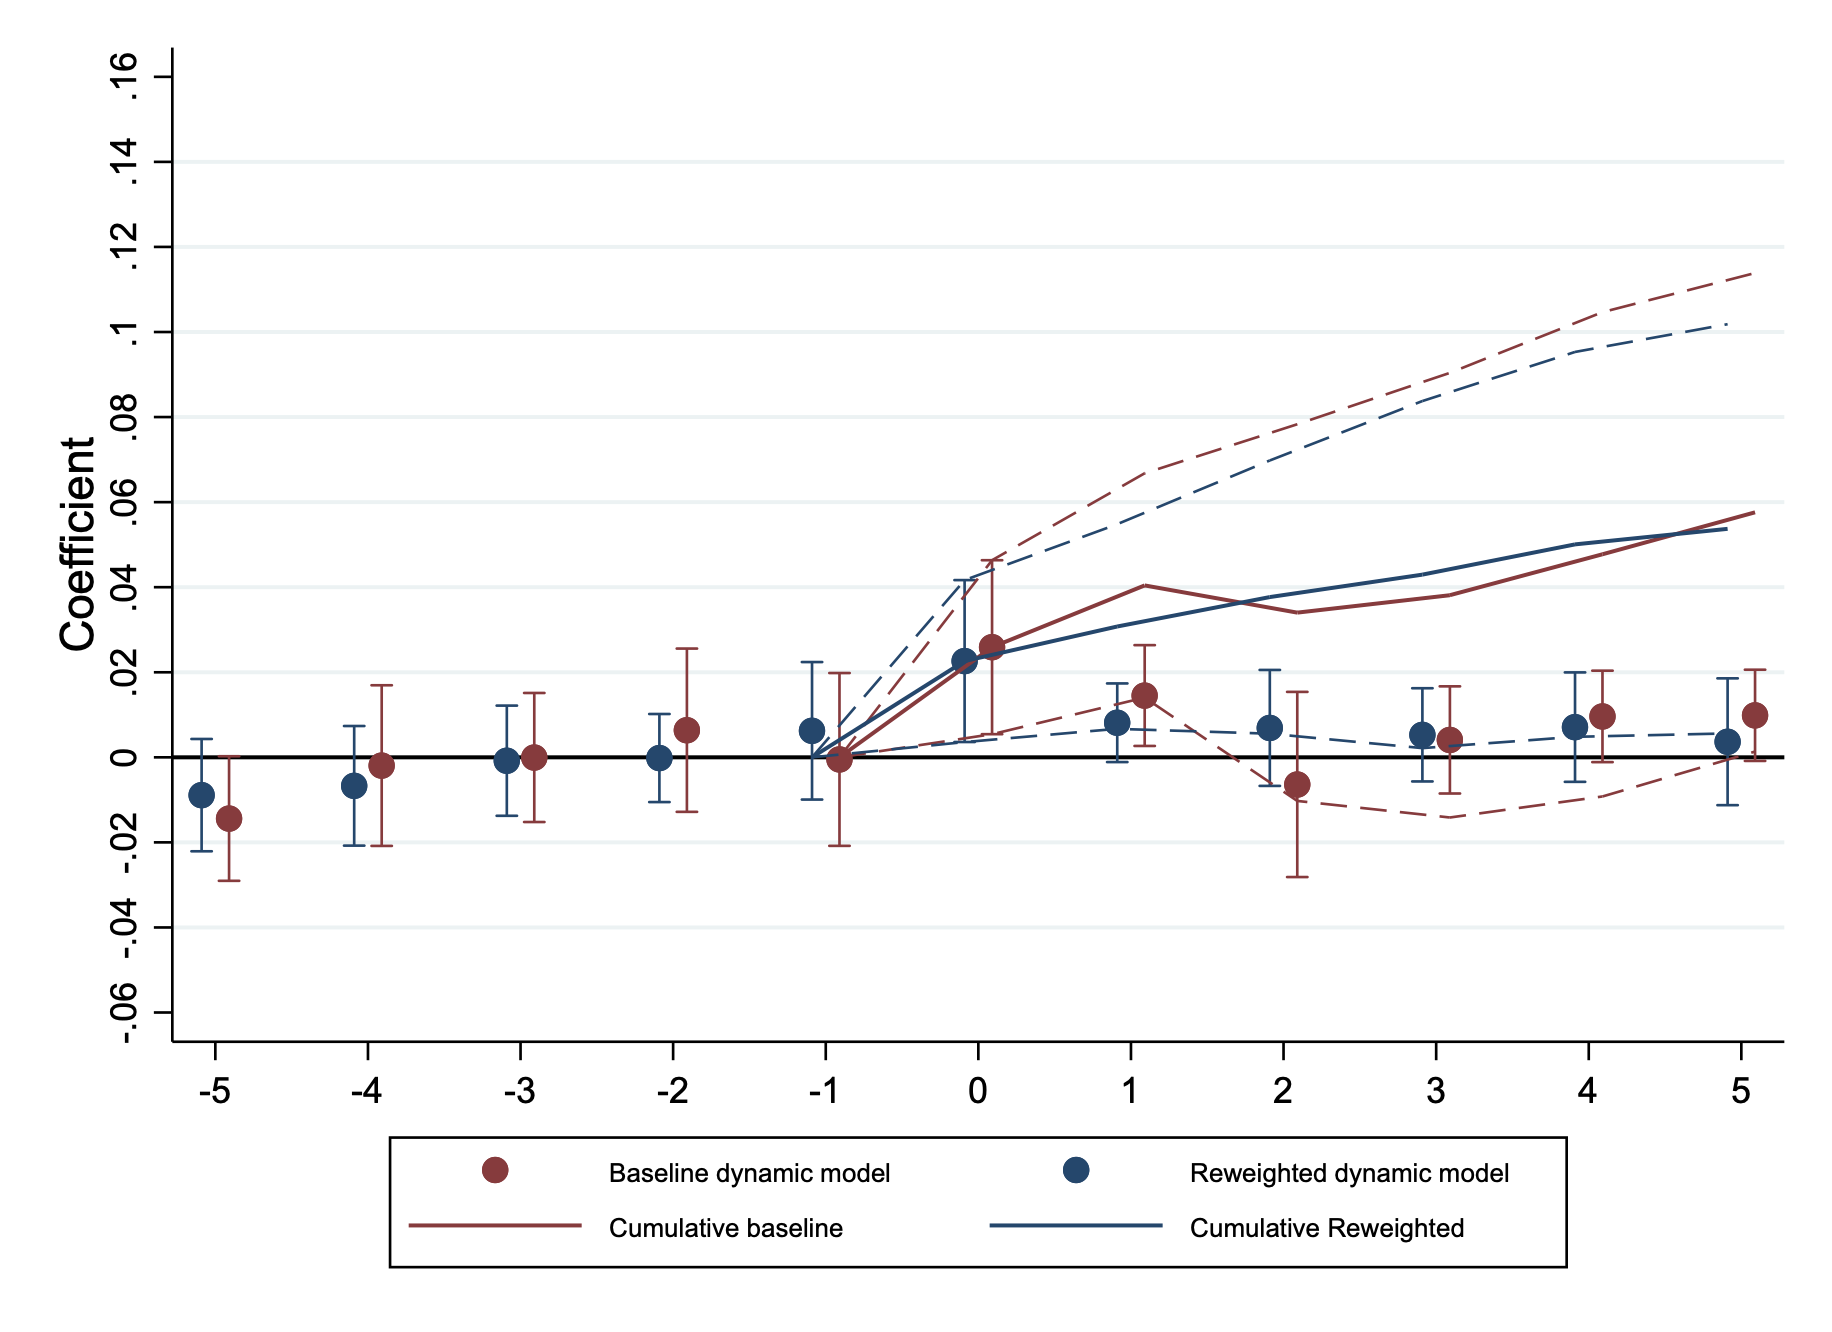
\includegraphics[width = \textwidth]
        {../../analysis/first_differences_unbal/output/fd_model_comparison_unbal.png}
    \end{subfigure}
    \begin{subfigure}[b]{0.8\textwidth}
        \caption{Reweighted panel}
        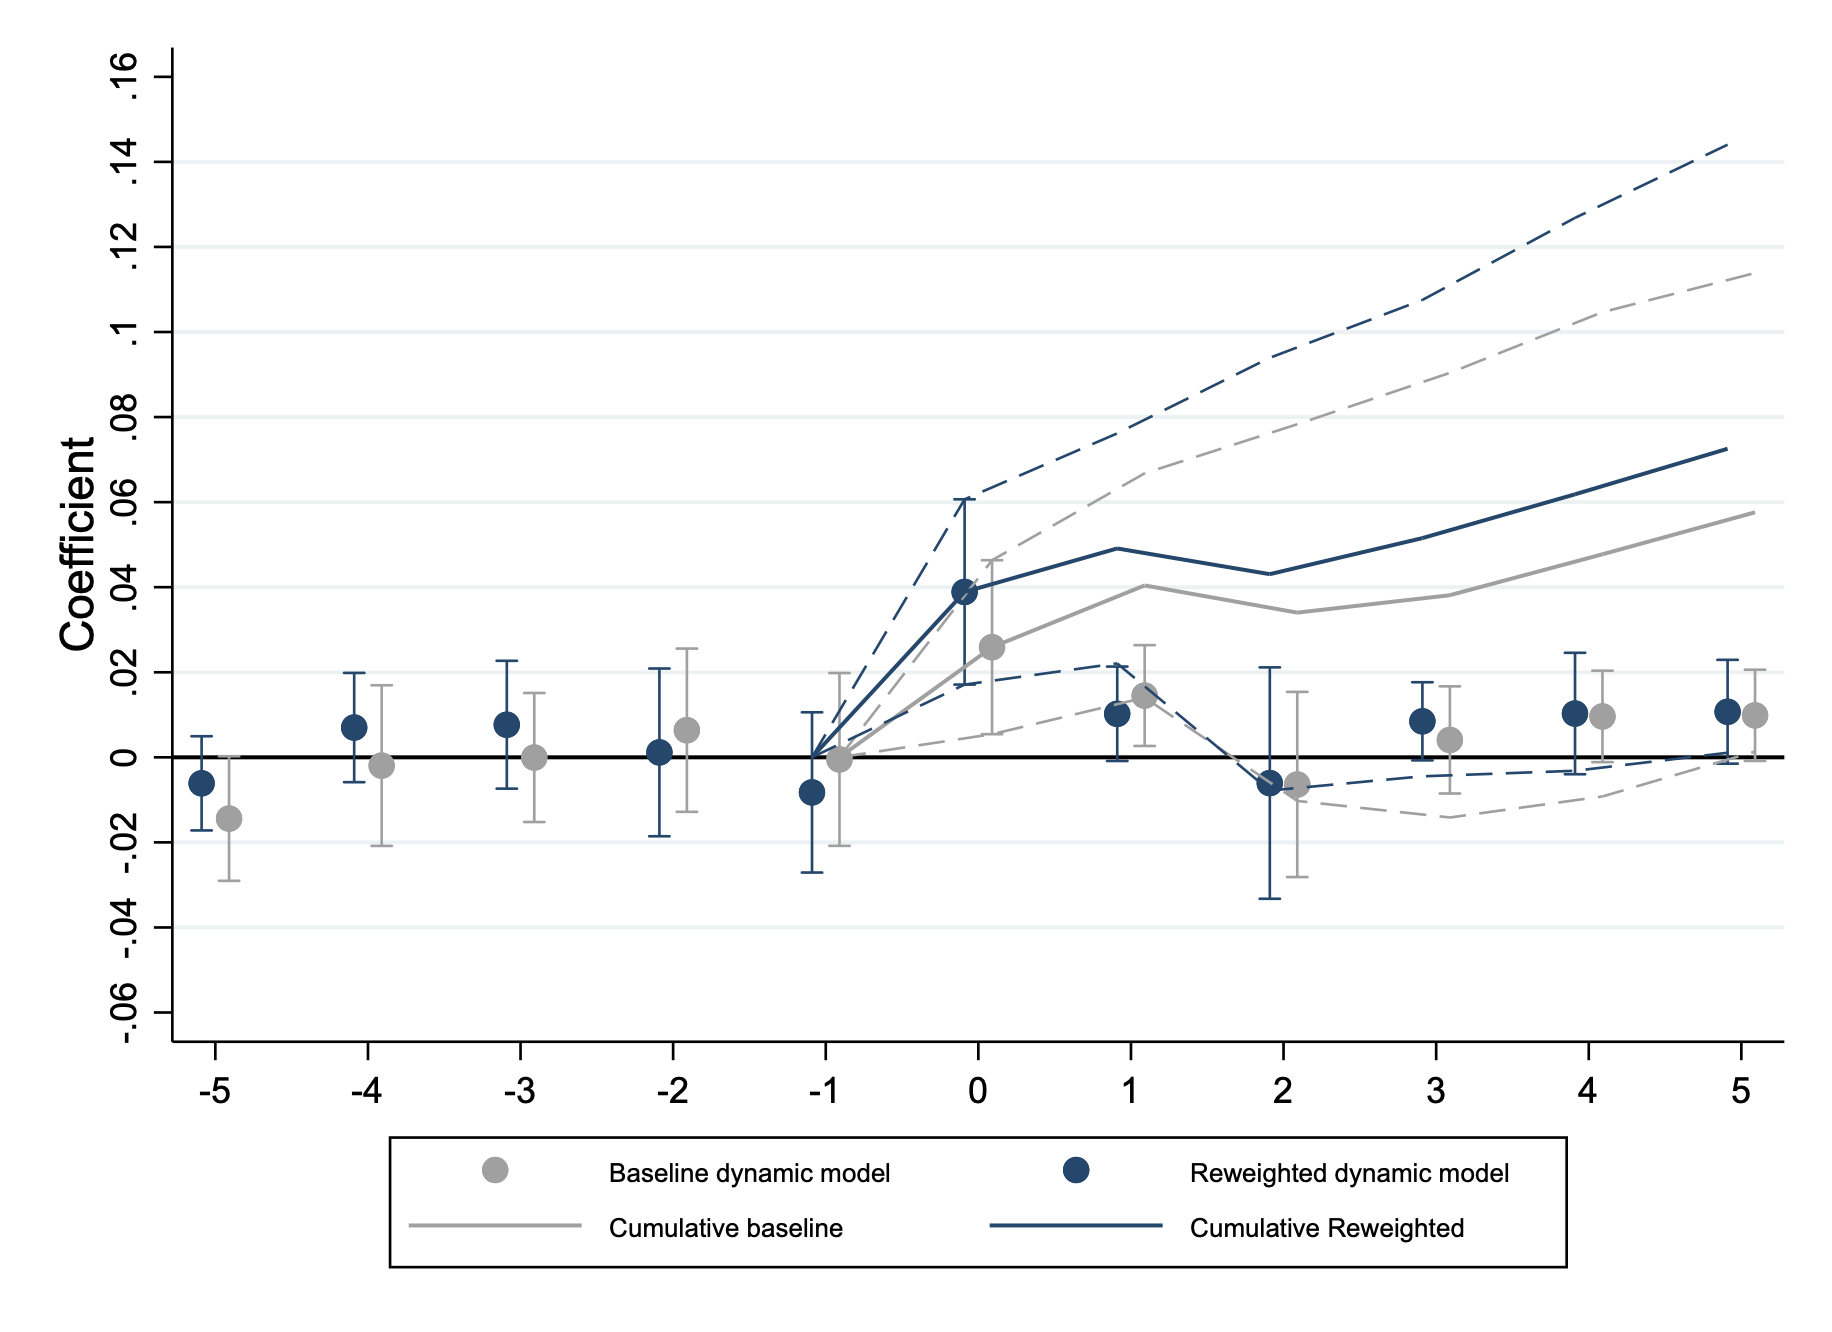
\includegraphics[width = \textwidth]
        {../../analysis/first_differences_wgt/output/fd_model_comparison_wgt.png}
    \end{subfigure}
    \begin{minipage}{0.95\textwidth} \footnotesize
		\vspace{2mm} 
		\textit{Notes}: The plot compares results obtained from the baseline panel summarized in 
		\autoref{tab:desc_stats}, column 4 with those obtained from the full unbalanced panel (a), 
		and with the reweighted baseline panel (b). Each subfigure compares estimated coefficients 
		for the \textit{dynamic DiD} models calculated through \autoref{eq:leads_lags}, and point 
		estimates for the cumulative effect of MW on rents estimated through \autoref{eq:lags}.   
	\end{minipage}
\end{figure}


%%%%%%%%%%%%%%%%%%%%%%%%%%%%%%%%%%%%%%%%%%%%%%%%%%%%%%%%%%%%%%%%%%%%%%%%%%%%%%%%%
\subsection{The Role of Unobserved Local Shocks}\label{sec:econ_shocks}

In \autoref{sec:baseline_results} we used \autoref{eq:leads_lags} to establish the absence of 
significant pre-trends in rent dynamics. Another potential threat to the identification of the true 
causal effect might come from unobserved local shocks systematically affecting MW and rent changes. 
In order to account for that, we directly control for proxies of general economic shocks, as well as 
shocks related to the labor and housing markets aggregated at either the county-month or 
county-quarter level, while rents are defined at the zipcode-level. While this prevents us from 
studying the presence of zipcode-level time-varying confounding factors, it substantially strengthens 
the robustness of the estimated impact since the treatment is administered at city, county, or state 
level. In fact, if there are underlying factors affecting MW changes that also affect zipcode-level 
rents, they would likely arise from this larger geographic units.

Controls included in our regressions are the following. First, to account for local economic shocks, 
we use the county-quarter number of establishments by industry obtained from the QCEW (see 
\autoref{sec:data} for more details). We then proxy for local labor market dynamics with two sets 
of controls: county-quarter weekly average wage, and county-month employment by industry. Since we 
are using a first-difference specification, we augment each model with their log difference. Second, 
we proxy for shocks that may stem from the housing market using the county-month number of new 
permits for residential one-unit buildings and the associated permits' valuation. Since these two 
series already report changes between periods, we only control for the log levels.

%\begin{table}[h!]
%    \caption{Results from Difference-in-Differences model with leads and lags and controls}
%    \label{tab:dynamic_leads_lags_econshock}
%    \centering
%    \resizebox{0.9\textwidth}{!}{
%	    \vspace{0pt}
%	    {
\def\sym#1{\ifmmode^{#1}\else\(^{#1}\)\fi}
\begin{tabular}{l*{5}{c}}
\hline\hline
          &\multicolumn{1}{c}{(1)}&\multicolumn{1}{c}{(2)}&\multicolumn{1}{c}{(3)}&\multicolumn{1}{c}{(4)}&\multicolumn{1}{c}{(5)}\\
          &\multicolumn{1}{c}{D.ln\_med\_rent\_psqft}&\multicolumn{1}{c}{D.ln\_med\_rent\_psqft}&\multicolumn{1}{c}{D.ln\_med\_rent\_psqft}&\multicolumn{1}{c}{D.ln\_med\_rent\_psqft}&\multicolumn{1}{c}{D.ln\_med\_rent\_psqft}\\
\hline
F5D.ln\_mw &  -0.0157         &  -0.0150\sym{*}  &  -0.0150\sym{*}  &  -0.0146\sym{*}  &  -0.0191\sym{*}  \\
          &(0.00938)         &(0.00832)         &(0.00816)         &(0.00823)         &(0.00983)         \\
[1em]
F4D.ln\_mw & -0.00382         & -0.00125         & -0.00131         & -0.00114         & -0.00776         \\
          & (0.0101)         &(0.00874)         &(0.00875)         &(0.00873)         &(0.00938)         \\
[1em]
F3D.ln\_mw &-0.000214         & -0.00150         & -0.00179         & -0.00133         &  0.00420         \\
          &(0.00831)         &(0.00889)         &(0.00910)         &(0.00885)         &(0.00917)         \\
[1em]
F2D.ln\_mw &  0.00477         &  0.00200         &  0.00219         &  0.00263         &  0.00276         \\
          & (0.0115)         & (0.0115)         & (0.0116)         & (0.0117)         & (0.0133)         \\
[1em]
FD.ln\_mw  & -0.00143         & -0.00398         & -0.00397         & -0.00394         &  -0.0114         \\
          & (0.0142)         & (0.0146)         & (0.0145)         & (0.0145)         & (0.0167)         \\
[1em]
D.ln\_mw   &   0.0260\sym{**} &   0.0265\sym{**} &   0.0269\sym{**} &   0.0258\sym{**} &   0.0267\sym{*}  \\
          & (0.0110)         & (0.0113)         & (0.0108)         & (0.0105)         & (0.0140)         \\
[1em]
LD.ln\_mw  &   0.0118         &   0.0108         &   0.0112         &   0.0115         &   0.0169\sym{**} \\
          &(0.00805)         &(0.00834)         &(0.00859)         &(0.00878)         &(0.00752)         \\
[1em]
L2D.ln\_mw & -0.00884         & -0.00554         & -0.00561         & -0.00548         & -0.00101         \\
          & (0.0124)         & (0.0126)         & (0.0127)         & (0.0127)         & (0.0143)         \\
[1em]
L3D.ln\_mw &  0.00191         &  0.00324         &  0.00326         &  0.00453         &  0.00845         \\
          &(0.00812)         &(0.00821)         &(0.00829)         &(0.00795)         &(0.00837)         \\
[1em]
L4D.ln\_mw &  0.00918         &   0.0105         &   0.0108         &  0.00968         &   0.0105         \\
          &(0.00724)         &(0.00686)         &(0.00680)         &(0.00683)         &(0.00675)         \\
[1em]
L5D.ln\_mw &  0.00736         &  0.00743         &  0.00749         &  0.00748         &  0.00702         \\
          &(0.00717)         &(0.00785)         &(0.00782)         &(0.00775)         &(0.00834)         \\
\hline
P-value no pretrends&    0.602         &    0.632         &    0.609         &    0.633         &    0.514         \\
Industry-level monthly employment&       No         &      Yes         &      Yes         &      Yes         &      Yes         \\
Industry-level quarterly establishment count&       No         &       No         &      Yes         &      Yes         &      Yes         \\
Industry-level quarterly weekly wage&       No         &       No         &       No         &      Yes         &      Yes         \\
New housing permits and value&       No         &       No         &       No         &       No         &      Yes         \\
R-squared &    0.027         &    0.028         &    0.028         &    0.028         &    0.031         \\
Observations&   106446         &   101448         &   101448         &   101448         &    82716         \\
\hline\hline
\end{tabular}
}
}
%    \begin{minipage}{0.95\textwidth} \footnotesize
%		\vspace{3mm} 
%		\textit{Notes}: The table reports coefficients from \autoref{eq:leads_lags} estimated on the 
%		balanced panel of zipcode-months that contains SFCC rental price. All specifications include 
%		zipcode linear trends. Column (1) replicates our baseline results from 
%		\autoref{tab:dynamic_lags_leads_main}, column 2. Columns 2 to 5 progressively add sets of 
%		time-varying covariates that control for local shocks. Columns 2 to 4 add controls for the 
%		following industries: goods-producing; natural resources and mining; construction; 
%		manufacturing; service-providing; trade, transportation and utilities; information; 
%		financial activities; professional and business services; education and health services; 
%		leisure and hospitality. They additionally control for federal, state, and local government. 
%		Standard errors clustered at the state level. *** $p < 0.01$, ** $p < 0.05$, * $p < 0.1$.
%	\end{minipage}
%\end{table}

In \autoref{tab:dynamic_leads_lags_econshock} we report the estimated coefficients for 
\autoref{eq:leads_lags}, progressively increasing the set of controls included in the regression. 
Column 1 replicates our baseline results (\autoref{tab:dynamic_lags_leads_main}, column 2); columns 
2 to 5 show estimated coefficients when adding all the aforementioned covariates. The estimated 
impact of MW changes remains substantially unchanged regardless of the set of controls used: we 
consistently observe that a 10 percent increase in MW causes a simultaneous increase in rents of 
approximately 0.26 percent. Only in column 5 we cannot reject the null hypothesis that 
$\hat{\beta}_{t} = 0$, as the points estimate slightly decreases while the smaller sample size 
leads to higher standard errors, but the coefficient on $t+1$ is also larger and significant. A 
quick comparison with leads and lags however clearly indicates the unchanged nature of our results. 
The inclusion of this relevant controls reveals the presence of a very mild pre-trend, however, we 
note that the joint F-test on all leads still fails to reject that they are all zero.   


%%%%%%%%%%%%%%%%%%%%%%%%%%%%%%%%%%%%%%%%%%%%%%%%%%%%%%%%%%%%%%%%%%%%%%%%%%%%%%%%%
\subsection{The Heterogeneity of MW Impacts on Rents}\label{sec:heter}

Our baseline results in \autoref{sec:baseline_results} have documented the presence of a causal 
impact of MW on rents, and the effect appears robust to multiple checks introduced in Sections 
\ref{sec:sample_rest} and \ref{sec:econ_shocks}. We now investigate the heterogeneity of such effect 
by characterizing zipcodes based on socio-demographic characteristics. The goal of this exercise is 
twofold: first, MW is a place-based policy targeted to a specific sub-population that does not 
necessarily live and work in the same zipcode. The presence of a significant effect in treated 
zipcodes does not reveal whether MW workers are actually bearing the burden of this increase, or if 
instead rents increase in those zipcodes where MW jobs are concentrated. We therefore try to answer 
the following question: do rents increase more where MW workers live, or where they work? second, 
independently from the incidence on MW workers, who are the winners and losers when rents increase 
due to new MW provisions? we look at zipcode characteristics to identify which sub-population ends 
up paying more in rents.

To answer the first question it requires to localize MW workers job and residence locations at the 
zipcode level. While direct data on this feature of zipcodes is not available, we build proxies 
based on the LODES data. Specifically, we use the 2017 files to compute the share (out of state 
totals) of low-income workers under 30 years old that either live or work in any given zipcodes (MW 
workplace and residence distribution henceforth).\footnote{See \autoref{sec:data} for more details 
	on the construction of such variables.} 
Since the majority of the MW changes in our data are at the state-level, we calculate shares over 
state totals so that we are able to study the impact of this type of policy on the relevant 
distribution of low-income, young workers. While these proxies by definition include more than MW 
workers, \cite{dube2016minimum} show how MW changes actually affect a larger part of the income 
distribution than just workers below MW thresholds (a statistically significant impact on wages is 
reported up to $\$4$ above the new MW thresholds). We then bin each state distribution into quartiles 
and use \autoref{eq:diff_main_hetero} to estimate the differential effect for each group.

\begin{figure}[h!]
    \caption{Static DiD model: MW impact by workers job and residence location}
    \label{fig:static_dd_workers_home_work}
    \centering
    \begin{subfigure}[b]{0.6\textwidth}
        \caption{Workplace location}                  %%% CHANGE INPUT FOLDER
        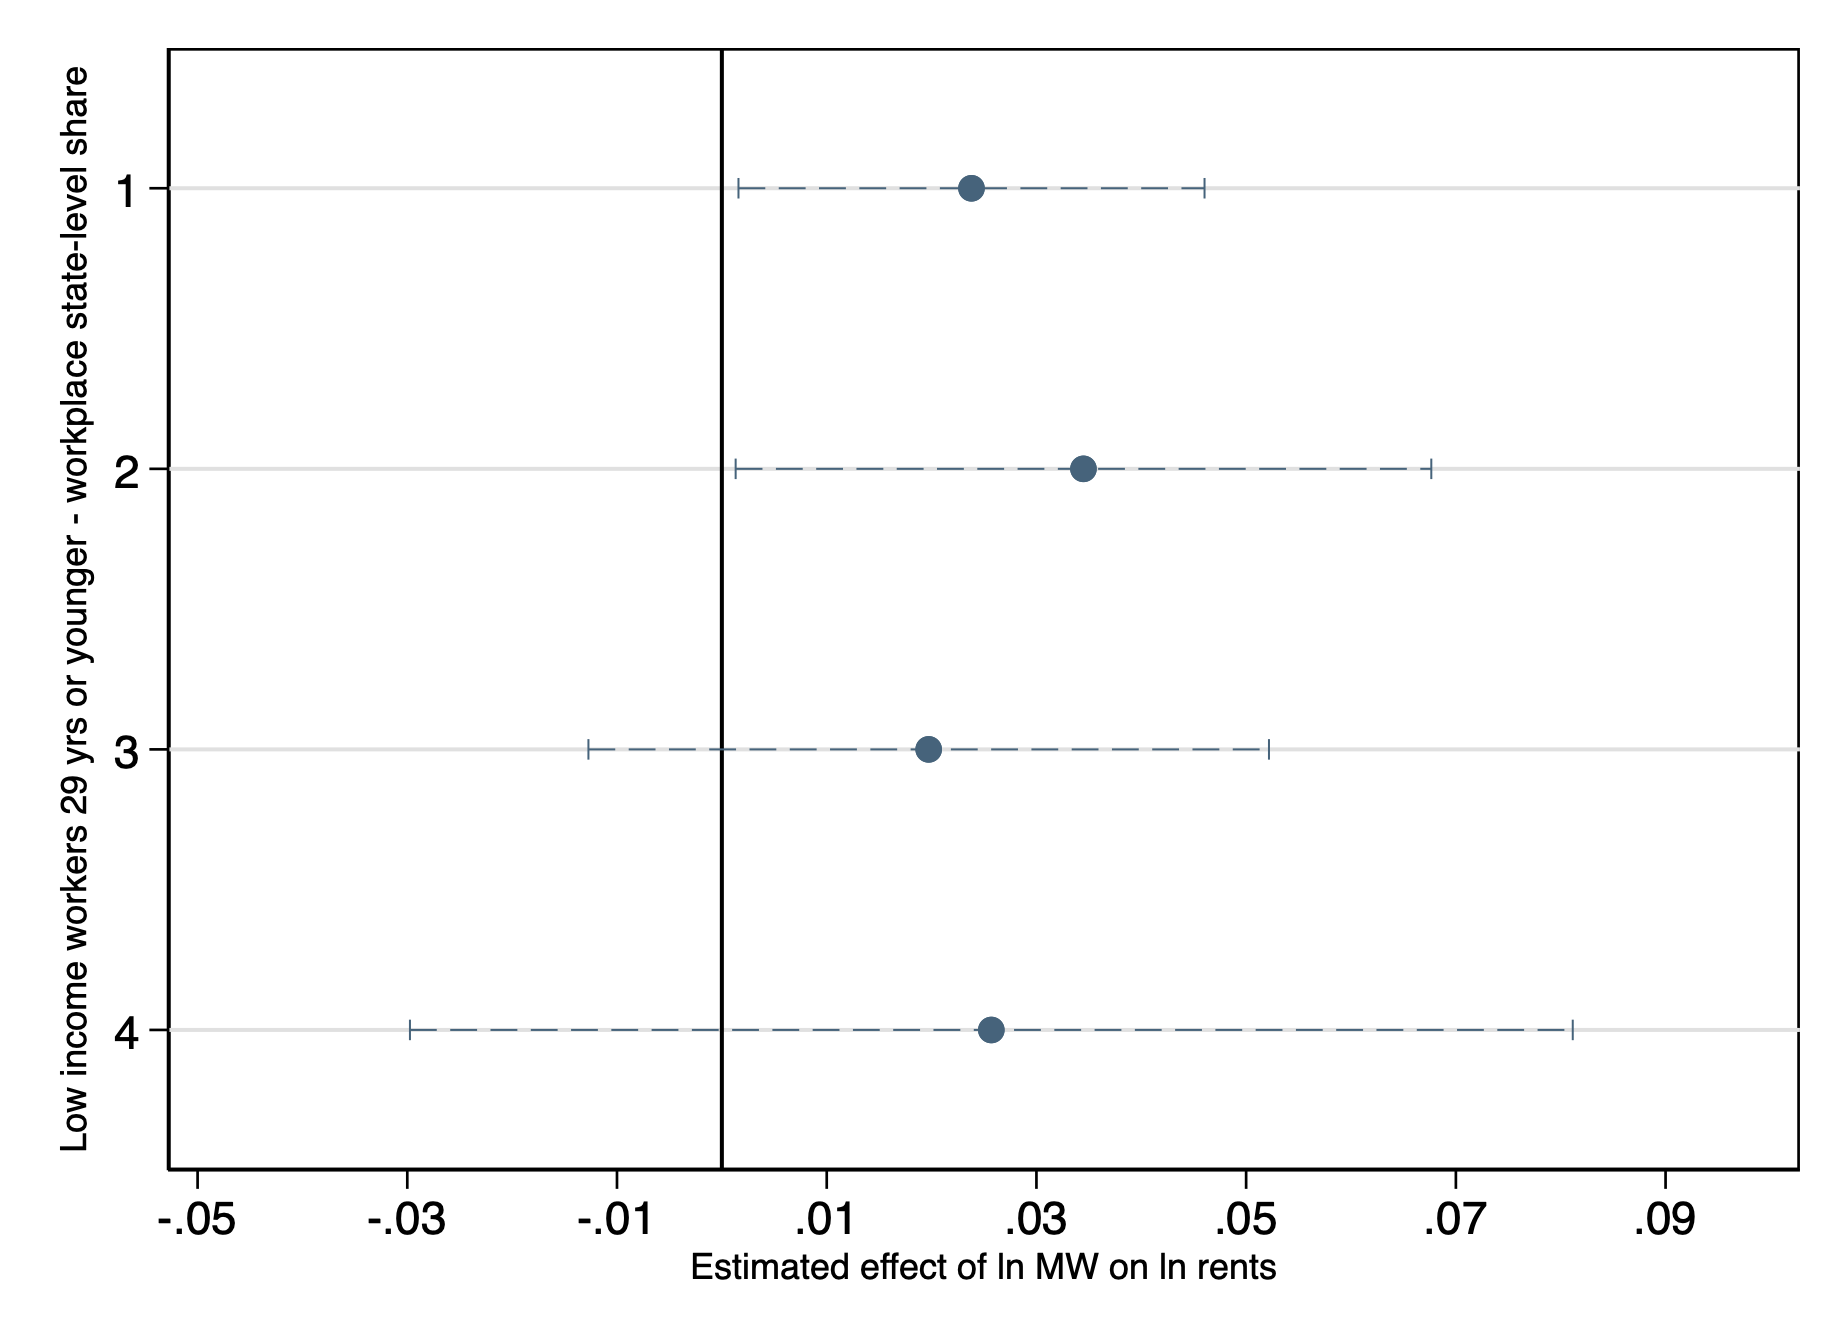
\includegraphics[width = \textwidth]{../input/fd_static_heter_walall_29y_lowinc_ssh.png}
    \end{subfigure}
    \begin{subfigure}[b]{0.6\textwidth}
        \caption{Residence location}
        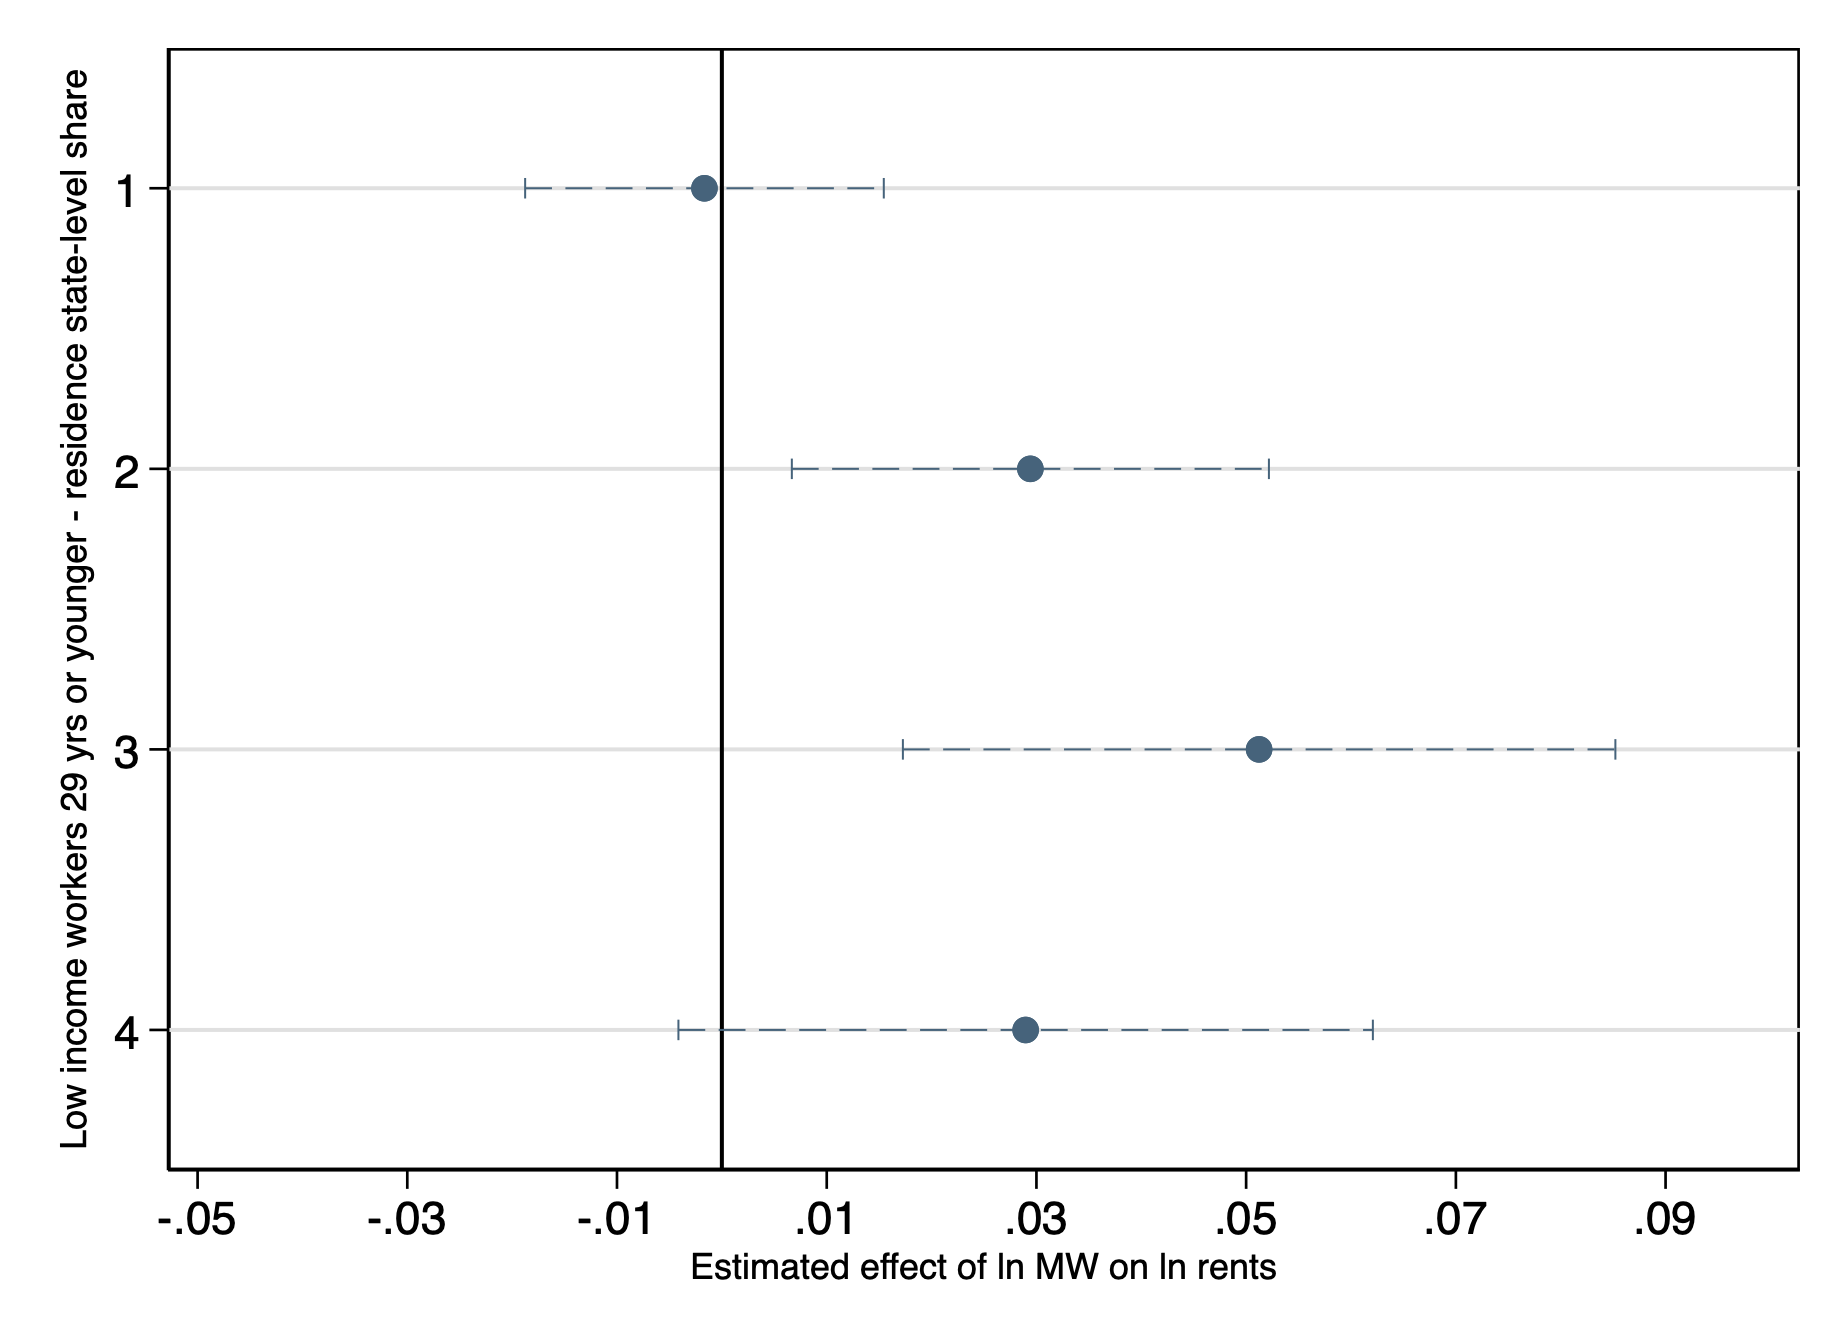
\includegraphics[width = \textwidth]{../input/fd_static_heter_halall_29y_lowinc_ssh.png}
    \end{subfigure}
    \begin{minipage}{0.95\textwidth} \footnotesize
		\vspace{2mm} 
		\textit{Notes}: The Figure shows the estimated coefficients $\beta_{q}$, $q \in \{1, 2, 3,
		4\}$ from \autoref{eq:diff_main_hetero} when differentiating zipcodes with respect to the 
		share of MW workers that either work (a) or live (b) in each zipcode. Shares are taken over 
		state totals. MW workers is used as a loose label for workers below 30 years old earning 
		less than $\$1250$ month identified using the 2017 LODES datasets (see \autoref{sec:data} 
		for more information). 90 percent confidence intervals reported.
	\end{minipage}
\end{figure}

In \autoref{fig:static_dd_workers_home_work} we plot the estimated coefficients for the interaction 
between changes in (log) MW and each quartile of the two distributions. Panel (a) presents results 
for MW workplace location. The point estimates are very similar, suggesting that the effect on rents 
is orthogonal to the geographic distribution of MW workplace. The coefficients for the first 2 
quartiles are significant at the $10$ percent level, but standard errors for the $3^{rd}$ and 
$4^{th}$ quartiles become very large partly due to a heavily right-skewed distribution of the 
underlying variable. In panel (b) we re-estimate \autoref{eq:diff_main_hetero} using the MW residence 
distribution. Here we do observe a different pattern: the point estimate in the lowest quartile is 
precisely zero, but this increases and becomes statistically significant both in the $2^{nd}$ and 
$3^{rd}$ quartile. Even more, the effect appears larger: a 10 percent increase in MW leads to a 0.5 
percent increase in rents. The estimated effect for zipcodes with the highest share of young, 
low-income workers decreases to 0.3 percent and becomes not significant, but we notice how also the 
underlying MW residence distribution is heavily right-skewed, and this higher variance partially 
justify the lower precision in our estimates. Overall, this exercise shows how MW workers indeed seem 
to bear most of the impact with relatively higher rents in their place of residence.

The LODES-based proxies for MW workers are approximate by definition. We then turn to investigate 
how the impact of MW changes on rents differs across the distribution for different census-based 
zipcode demographics. The Bureau of Labor Statistics reports how MW workers tend to be young and 
less educated.\footnote{See, for example, BLS Report 1085, \textit{Characteristics of Minimum Wage 
		Workers 2019}.} % Link: \url{https://www.bls.gov/opub/reports/minimum-wage/2019/home.htm}
The study of heterogeneous effects by demographics can therefore help both in confirming what the
LODES-based measures indicate, and in uncovering additional patterns of the effects under study.

\autoref{tab:fd_model_het} shows the estimated coefficients for the interaction between changes in 
(log) MW and quartiles of the distribution for several demographics. In column 1 we show how the 
effect disproportionately impact zipcodes in the lowest quartile of the median income distribution: 
the estimated elasticity of rent to MW is 0.039 (s.e. 0.022). The effect on the other quartiles 
becomes not significant and it shows a non-monotone behavior in the $2^{nd}$ and $3^{rd}$ quartiles. 
When looking at the richest neighborhoods however, we have a markedly smaller and imprecise estimate. 
In column 2 we focus on the zipcode-level unemployment  rate. Not surprisingly, we find that the 
strongest effect is localized in the $4^{th}$ quartile of the distribution, 0.045 (s.e. 0.017). 
Estimates lose significance in the remaining part of the distribution: similarly to column 1, we 
find not-significant not-monotone estimates in the middle quartiles, while the effect is a clear 
zero in the bottom quarter. In column 3 we look at the share of college graduates, and the estimates 
confirm that indeed lower educated neighborhoods bear the bulk of the rent increase: there is a 
clear divide between above median zipcodes showing zero and not significant effects, and below 
median ones where a 10 percent increase in MW leads to a 0.47 and a 0.37 percent rent increase for 
the $2^{nd}$ and $1^{st}$ quartiles, respectively. Lastly, in column 4 we show the impact across 
the distribution over share of African-American residents. Similarly to column 3, we do find a 
stark contrast between above and below median zipcodes. The effect of MW changes on rents 
monotonically increases starting from a not significant effect of 0.017 in the $1^{st}$ quarter to 
a statistically significant 0.042 in the $4^{th}$ one.

\begin{table}[h!]
    \caption{Heterogeneity Results - static DiD model}
    \label{tab:fd_model_het}
    \centering
    \resizebox{0.9\textwidth}{!}{             %%% CHANGE INPUT FOLDER
	    \vspace{0pt}    
	    {
\def\sym#1{\ifmmode^{#1}\else\(^{#1}\)\fi}
\begin{tabular}{l*{6}{c}}
\hline\hline
          &\multicolumn{1}{c}{(1)}&\multicolumn{1}{c}{(2)}&\multicolumn{1}{c}{(3)}&\multicolumn{1}{c}{(4)}&\multicolumn{1}{c}{(5)}&\multicolumn{1}{c}{(6)}\\
          &\multicolumn{1}{c}{\shortstack{Median \\ income}}&\multicolumn{1}{c}{\shortstack{College \\ grad. (\%)}}&\multicolumn{1}{c}{\shortstack{15-24 years \\ old (\%)}}&\multicolumn{1}{c}{\shortstack{African- \\ am. (\%)}}&\multicolumn{1}{c}{\shortstack{Young \\ low-inc. worker,\\ workplace}}&\multicolumn{1}{c}{\shortstack{Young \\ low-inc. worker,\\ residence}}\\
\hline
First quartile&   0.0373         &   0.0356\sym{*}  &   0.0196         &   0.0175         &   0.0214         & -0.00317         \\
          & (0.0223)         & (0.0197)         & (0.0139)         & (0.0159)         & (0.0131)         &(0.00981)         \\
[1em]
Second quartile&   0.0193         &   0.0448\sym{**} &   0.0187         &   0.0217         &   0.0340\sym{*}  &   0.0304\sym{**} \\
          & (0.0146)         & (0.0217)         & (0.0156)         & (0.0157)         & (0.0194)         & (0.0128)         \\
[1em]
Third quartile&   0.0300         &   0.0255         &   0.0212         &   0.0209         &   0.0196         &   0.0498\sym{**} \\
          & (0.0245)         & (0.0208)         & (0.0149)         & (0.0132)         & (0.0187)         & (0.0201)         \\
[1em]
Fourth quartile&   0.0129         &-0.000230         &   0.0414\sym{***}&   0.0404\sym{**} &   0.0249         &   0.0268         \\
          & (0.0126)         & (0.0114)         & (0.0144)         & (0.0162)         & (0.0330)         & (0.0197)         \\
\hline
P-value equality&    0.813         &    0.176         &    0.230         &    0.487         &    0.768         &    0.005         \\
Observations&  107,781         &  107,781         &  107,781         &  107,781         &  107,568         &  107,707         \\
\hline\hline
\end{tabular}
}

    }
    \begin{minipage}{0.95\textwidth} \footnotesize
		\vspace{3mm}
		\textit{Notes}: The table reports estimates for $\beta_{q}$, $q=\{1, 2, 3, 4\}$ from 
		\autoref{eq:diff_main_hetero} when differentiating zipcodes based on several 
		socio-demographics from the 2010 Census and the 5-year 2008-2012 ACS. Standard errors 
		clustered at the state level. *** $p < 0.01$, ** $p < 0.05$, * $p < 0.1$.  
	\end{minipage}
\end{table}
